\chapter{Results}\label{ch:cfd}
\begin{em}
Intro
\end{em}
\section{Benchmarking}
To check my method, the results can be benchmarked against a known solution. For this, we turn to Sch\"onhammer's solution for the 1D linear harmonic oscillator. This was previously considered in Section 1.4 and has an exact solution given by equations (1.31) and (1.32). Applying my method, the results can be plotted on top of the exact solution as shown in Fig. (3.1). It is more useful to show the difference as seen in Fig. (3.2). 

There are two important parts of Fig. (3.2) that are worth noting. The first is the scale of the y-axis. This is the difference between the Sch\"onhammer's exact solution and the program solution. The range of $10^{-8}$ is important to note because this was the precision parameter that was set in the code. If a higher level of accuracy is required in this calculation, the precision can easily be changed.  

\begin{figure}[H]
    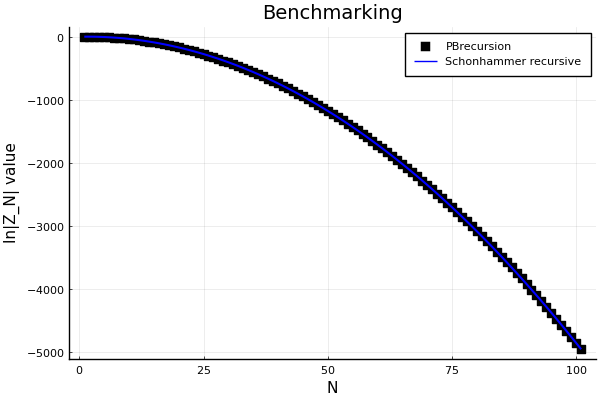
\includegraphics[scale=0.75]{figures/pdf/Benchmarking.png}
    \caption{Solution from Poisson Binomial recursive method versus the Sch\"onhammer exact solution}
\end{figure}

\begin{figure}[H]
    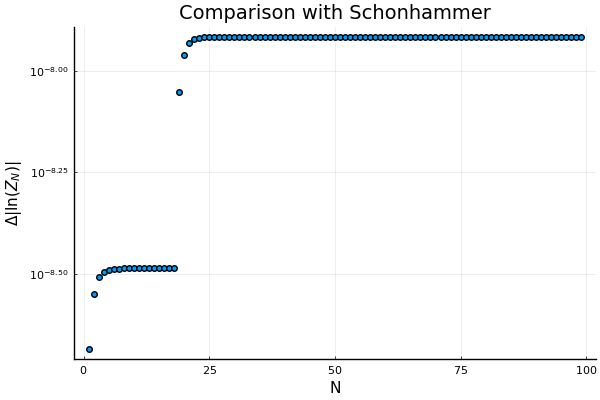
\includegraphics[scale=0.75]{figures/pdf/Benchdiff.png}
    \caption{Difference between the logarithms of the Poisson Binomial solution and the Sch\"onhammer solution}
\end{figure}

The other part to note is the jump in the error. This is due to the process of building the initial occupation probability distribution. As a reminder, the program is dealing with a fixed number of particles at ultra-low temperatures. At these temperatures, only the region around the Fermi level will have any sort of probability away from one or zero. Therefore, to increase the speed of the calculation, the states that are above a cutoff value are certain to be occupied. For these states with occupation probability of one, a counter keeps track of the number of particles and their probabilities are not included in the distribution. Similarly, any probability that is below the cutoff is not included because it is taken to have a zero probability of being occupied. This process saves memory and makes the calculations throughout the program much faster. The downside to this process is that a small error is introduced. This is the source of the jump shown in Fig. (3.2). At this point, energy levels are left out of the distribution. Again, the error is controllable based on the precision chosen by the user.

\section{Controlling Chemical Potential}
The key role of the chemical potential is to ensure that the grand canonical ensemble has the correct number of particles in the system. The correct choice in chemical potential will effect the error of the measurement. Therefore, it's necessary to choose $\mu$ such that 
\begin{equation}
    N=\sum_i \avg{p_i}=\sum_i \frac{e^{-\beta(E_i-\mu)}}{Z_{GC}}
\end{equation}
where $N$ is the number of particles in the system. In the previous section, the partition function was calculated for different values of $N$. For each of these calculations, the choice in chemical potential is different. One interesting question is how much does this choice in chemical potential effect the error when calculating the partition function. To inspect this, we can set the chemical potential to a value and proceed with the same benchmarking code. The results of this are shown in Figure (3.3). We can see that the correct chemical potential will provide a minimum at its corresponding particle number value. After that, it increases as some absolute value of the distance from the correct $N$ value. Therefore, it's necessary that the chemical potential be updated each step in order to keep the errors at the minimum. 

\begin{figure}[H]
    \centering
    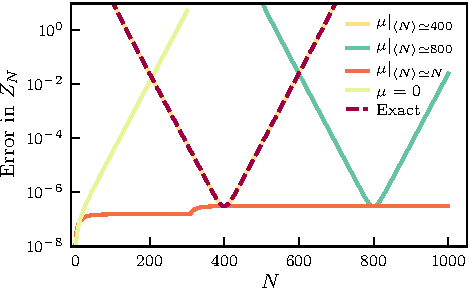
\includegraphics[scale=1.5]{figures/pdf/Plot1.pdf}
    \caption{Errors from fixed $\mu$}
    \label{fig:Errors}
\end{figure}

\section{Numerical results of nondegenerate spectra}
In this section, we will consider the case where our spectrum is nondegenerate. From the Section (1.3), we expect that the error of the temperature measurement $\beta^*$ in the grand canonical ensemble should reach $100\%$ once $\beta$ get sufficiently large enough. We also saw the same result in Section (2.5) when we set $g_0=g_1=g_{-1}=...=1$ in equation (2.66). Now I will show how the code reproduces these results. The two spectra I consider are the simple harmonic oscillator (linear spectrum) and the potential well spectrum (quadratic spectrum). The results of my program are shown in Figures (3.4) and (3.5) where the y-axis is $\frac{\delta\beta}{\beta}=\frac{\beta^*-\beta}{\beta}$. An interesting difference between the two figures is length of the x-axis. The linear spectrum reaches $100\%$ error slower than the quadratic error. This is due to the spacing between energy levels. For the linear spectrum, this spacing is constant, while the quadratic spectrum has a spacing that linearly increases. This means that more energy is required to fill the first excited state for the quadratic spectrum as the number of particles increases. The spacing term $\Delta_0$ will always increase, and thus the Boltzmann probability $e^{-\beta\Delta_0}$ that the state is occupied will continually decrease. For this reason, it's more difficult to calculate the error for linear spectra. 

\begin{figure}[H]
    \centering
    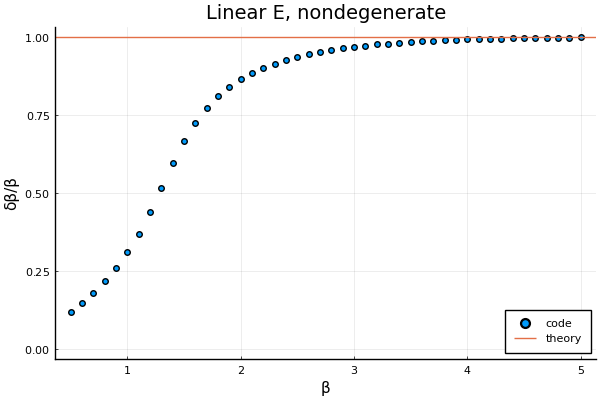
\includegraphics[scale=0.75]{figures/pdf/linEnondeg.png}
    \caption{Error in $\beta^*$ measurement nondegenerate Linear Energy spectrum}
    \label{fig:Error2}
\end{figure}

\begin{figure}[H]
    \centering
    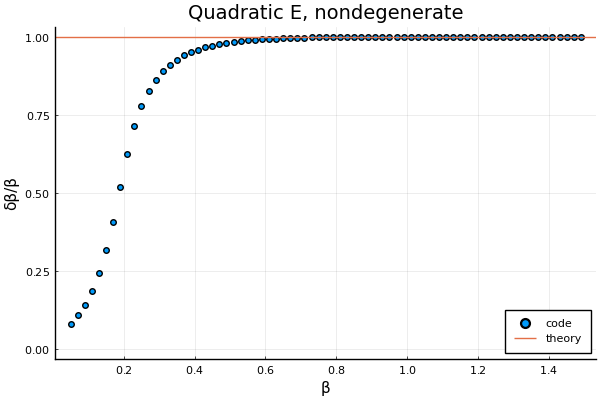
\includegraphics[scale=0.75]{figures/pdf/quadEnondeg.png}
    \caption{Error in $\beta^*$ measurement nondegenerate Quadratic Energy spectrum}
    % \label{fig:Error in $\beta^*$ measurement nondegenerate Quadratic Energy spectrum}
\end{figure}


\section{Numerical results of degenerate spectra}
In this section, we want to consider the spectra that are degenerate. Specifically, we want to verify the equations in Section (2.5). I will first consider the case where the Fermi level is filled and then consider the case of partial filling. Finally, I will provide a special case where the Fermi level is almost degenerate. 
\subsection{Filled Fermi Level}
To start, the Linear energy spectrum is used. Equation (2.66) are plotted on top of the results of the program in Figure (3.6).  

\begin{figure}[H]
    \centering
    \includegraphics[scale=0.75]{figures/pdf/linE_N10_filled_g0-2_Δ0-1.png}
    \caption{Filled Degenerate Linear Spectrum $\beta^*$ Error}
    \label{fig:Filled}
\end{figure}

We can see that the error follows the theory once $\beta$ is sufficiently large enough. To further inspect this, I will rewrite Equation (2.66) in the following way. 
\begin{align}
    \frac{\delta\beta}{\beta}&=1-\frac{\ln(g_0g_1)}{\Delta_0\beta}\\
    \frac{\delta\beta}{\beta}-1&=-\frac{\ln(g_0g_1)}{\Delta_0\beta}\\
    \beta\Delta_0-\delta\beta\Delta_0&=\ln(g_0g_1)
\end{align}
In this calculation, I have neglected the exponential term for convenience. Equation (3.4) is then plotted against the program as shown in Figure (3.7). 
\begin{figure}[H]
    \centering
    \includegraphics[scale=0.75]{figures/pdf/linE_N10_filled_g0-2_Δ0-1_1.png}
    \caption{Filled Degenerate Linear Spectrum Adjusted $\beta^*$ Error}
    \label{fig:FilledDegenerateLinearSpectrumAdjustedError}
\end{figure}
Again, we can see that at high enough $\beta$ the program aligns with the theory. 

Now I will consider the filled degenerate quadratic energy spectrum. The analysis will be the same, so Equation (3.4) will still be used. The results of the program are shown in Figures (3.8) and (3.9). 

\begin{figure}[H]
    \centering
    \includegraphics[scale=0.75]{figures/pdf/quadE_N10_filled_g0-2_Δ0-1.png}
    \caption{Filled Degenerate Quadratic Spectrum $\beta^*$ Error}
    \label{fig:FilledDegenerate}
\end{figure}

\begin{figure}[H]
    \centering
    \includegraphics[scale=0.75]{figures/pdf/quadE_N10_filled_g0-2_Δ0-1_1.png}
    \caption{Filled Degenerate Quadratic Spectrum Adjusted $\beta^*$ Error}
    \label{fig:FilledDegenerate2}
\end{figure}

Again, we can see that the program follows the trend of the theory. One note should be made for the slight variation at $\beta$ values of 1.5 or higher. The deviation is due to the cutoff that is used to determine the correct $\beta^*$ from Equation (2.30). Overall, however, the theory and program agree very well for filled degenerate energy spectra.

\subsection{Partially Filled Degenerate Energy Spectra}
Turning to the case of partial filling, we want to verify Equation (2.95). Again, I will start by considering the case of the simple harmonic oscillator first. The results are shown in Figure (3.10). 

\begin{figure}[H]
    \centering
    \includegraphics[scale=0.75]{figures/pdf/linE_N9_partfilled_g0-2_Δ0-1.png}
    \caption{Partially Filled Degenerate Linear Spectrum $\beta^*$ Error}
    \label{fig:PartiallyFilledDegenerateLinearSpectrum}
\end{figure}

We can see that there is pretty good agreement for large $\beta$ values. We can follow the same procedure as the filled spectrum and rewrite Equation(2.95).
\begin{align}
    \frac{\delta\beta}{\beta}&=\frac{1}{\beta\Delta_0}\ln(\frac{g_0-l+1}{g_0-l})\\
    \delta\beta \Delta_0&=\ln(\frac{g_0-l+1}{g_0-l})
\end{align}
Equation (3.6) can be plotted against the program data as seen in Figure (3.11). 

\begin{figure}[H]
    \centering
    \includegraphics[scale=0.75]{figures/pdf/linE_N9_partfilled_g0-2_Δ0-1_1.png}
    \caption{Partially Filled Degenerate Linear Spectrum Adjusted $\beta^*$ Error}
    \label{fig:PartiallyFilledDegenerateLinearSpectrumAdjustedError}
\end{figure}
We can see that the program is following the theory when $\beta$ is large enough. The dispersion of the tail of the data is due to the cutoff value like the deviation from Figure (3.8). Turning to the quadratic spectrum, the same calculations are plotted on Figures (3.12) and (3.13). 

\begin{figure}[H]
    \centering
    \includegraphics[scale=0.75]{figures/pdf/quadE_N9_partfilled_g0-2_Δ0-7.png}
    \caption{Partially Filled Degenerate Quadratic Spectrum $\beta^*$ Error}
    \label{fig:PartiallyFilledDegenerateQuadraticSpectrumError}
\end{figure}

\begin{figure}[H]
    \centering
    \includegraphics[scale=0.75]{figures/pdf/quadE_N9_partfilled_g0-2_Δ0-7_1.png}
    \caption{Partially Filled Degenerate Quadratic Spectrum Adjusted $\beta^*$ Error}
    \label{fig:PartiallyFilledDegenerateQuadraticSpectrumAdjustedError}
\end{figure}

The data follows the theory very will with the cutoff error still appearing after about $\beta=1$. Overall, the theory and data for the partially filled spectra agree very well. 
\subsection{Almost Degenerate Energy Spectrum}
For this section, I will consider the case where the spectrum is almost degenerate. From a theory standpoint, we expect that the error will follow the case of the partially filled theory until $\beta$ is large enough to break the pseudo-degeneracy. I will only consider the quadratic energy spectrum because the energy spacing will be large enough that any effects from this spectrum will be noticeable. 



\section{Other spectra}  
2D box trap with irrational ratio of lengths
